\documentclass[11pt,a4paper]{article}

\usepackage[english]{babel}
\usepackage[T1]{fontenc}
\usepackage[utf8]{inputenc}
\usepackage{graphicx}
\graphicspath{{../Figs/}}
\usepackage{float}
\usepackage{subcaption}
\usepackage[font=footnotesize,labelfont={sf,bf},textfont=sf,width=\textwidth]{caption}
\usepackage[margin=2cm]{geometry}
\usepackage[plainpages=false,pdfpagelabels,hypertexnames=false]{hyperref}
\usepackage[usenames,dvipsnames]{xcolor}
\usepackage{mathtools}
\usepackage[separate-uncertainty=true]{siunitx}
\usepackage{booktabs}


\title{\bfseries\textsc{Atomic Force Microscopy}}
\author{
Michele Masini\\ \small\texttt{\href{mailto:michele.masini@uni-ulm.de}{michele.masini@uni-ulm.de}}\and
Iyán Méndez Veiga\\ \small\texttt{\href{mailto:iyan.mendez-veiga@uni-ulm.de}{iyan.mendez-veiga@uni-ulm.de}}
}
\date{\today}


\begin{document}
\maketitle

\begin{abstract}
A compact Atomic Force Microscopy (AFM) from Nanosurf company (\href{https://www.nanosurf.com/en/products/naioafm-the-leading-compact-afm}{NaioAFM}) was used to perform measurements of the surface of three samples. Two different operation modes were used: static and tapping mode. Open source software \href{http://gwyddion.net/}{Gwyddion} was used to process the raw data.
\end{abstract}

\vspace{1.5cm}

\section{Introduction}

Since it was first developed in 1985 by \emph{Binning} et al., the Atomic Force Microscopy (AFM) \cite{Bhushan} has become a popular surface profiler for topographic and normal force measurements on the micro- to nanoscale. Not only AFMs, but also modified devices such as Lateral Force Microscopies (LFMs) or Friction Force Microscopies (FFMs), have found applications in different fields.

In this report, we will first describe the AFM technique, the two different operation modes that we tried (static and tapping or dynamic mode) and comment the issues we faced. And secondly, we will describe the processing of raw data obtained from the device using the open source software Gwyddion, as well as a general overview of AFM image artifacts, i.e., features which appear in the images that are not present in the original probed object.

\section{Materials and methods}

\subsection{AFM}

AFM relies on the same idea of Scanning Tunneling Microscope (STM), i.e., using a scanning technique to produce very high resolution, 3D images of sample surfaces. The difference is that instead of measuring tunneling currents, in AFM we measure ultrasmall forces between the tip surface and the sample surface to get the proximity of the tip to the sample, i.e., the height. This allows AFM to measure both conductors and insulators surfaces on an atomic scale.

By ultrasmall forces we mean forces of less than \SI{1}{\nano\N}. How this forces are measured is one of the key aspects of AFM because finding a relation between them and the distance between the tip and the surface will allow us to get a profile of the measured samples. However, this depends on the operation mode.

\begin{figure}[ht]
\centering
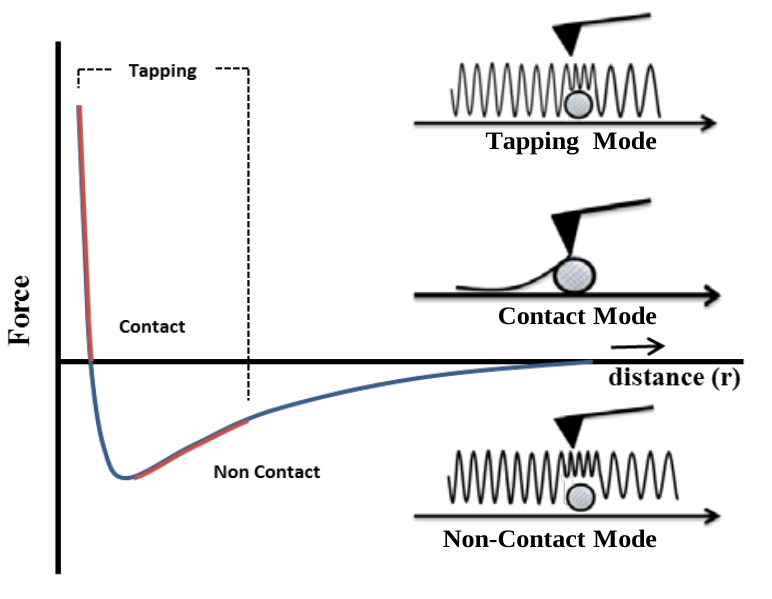
\includegraphics[width=0.7\textwidth]{AFM_modes}
\caption{Force that the tip experiments against the distance with respect to the surface of the sample \cite{jfb8010007}. In the contact mode forces are repulsive while in the non conntact mode are attractive. In the dynamic or tapping mode we are in between but typically in closer to the repulsive barrier.}
\label{fig:AFM_modes}
\end{figure}

{\color{red}Basically, we can say that AFM can be used in three modes or regimes} (see Figure \ref{fig:AFM_modes}): static, repulsive or contact mode; dynamic or tapping mode; and non-contact mode. In this report we will talk about the first two.

In the static mode, a sharp tip is brought into contact with the surface of the sample. The tip is placed at the end of a flexible (only in the normal direction) cantilever, which can deflect depending on the force that the tip ``feels''. The repulsive forces are due to electronic orbital overlap between the atoms of the tip and those in the surface of the sample. By measuring the deflection of the cantilever using tunneling, capacitive or optical detectors (see Figure \ref{fig:Deflection_measurement}), we can get a measure of the force if the cantilever spring constant is known.

\begin{figure}[ht]
\centering
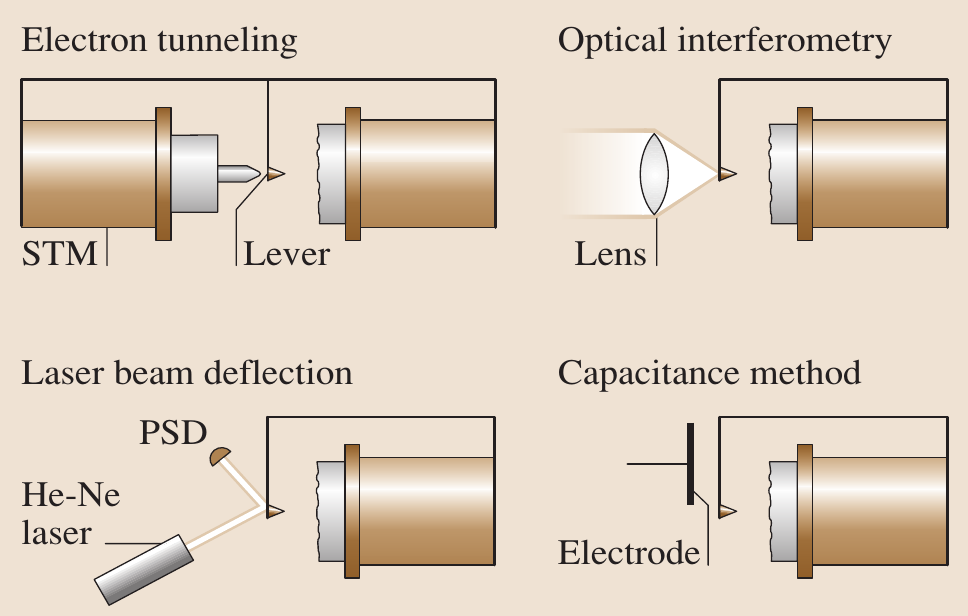
\includegraphics[width=0.5\textwidth]{Deflection}
\caption{Different techniques to measure cantilever deflection in an AFM \cite{Bhushan}.}
\label{fig:Deflection_measurement}
\end{figure}

The deflection can be measured to within \SI{0.02}{\nm}, so for a typical cantilever spring constant of \SI{10}{\N/\m}, forces as low as \SI{0.2}{\nano\N} can be measured.

Typically, the deflection of the cantilever is used as the signal for a feedback mechanism, so whenever due to the profile of the surface there is a change in this deflection, the distance $r$ between the tip and the surface of the sample is modified accordingly using a piezo material. The force that causes this aimed deflection is called \emph{setpoint} and we will see later that it is a key parameter when measuring in this mode. In order to get the profile of the whole surface, either the tip or the sample has to be translated using a piezoelectric scanner.

When we are on the right of the equilibrium (see Figure \ref{fig:AFM_modes}), the attractive forces on the tip are very weak van der Waals forces. Tapping mode can work on this regime but we do not measure the force anymore, but the force gradient. The cantilever is deliberately vibrated in either amplitude modulation (AM) or frequency modulation (FM) at its resonant frequency $\omega_0$ given by the spring constant and the force derivative is determined by measuring the shift in this resonant frequency due to the interaction with the sample.

\begin{figure}[ht]
\centering
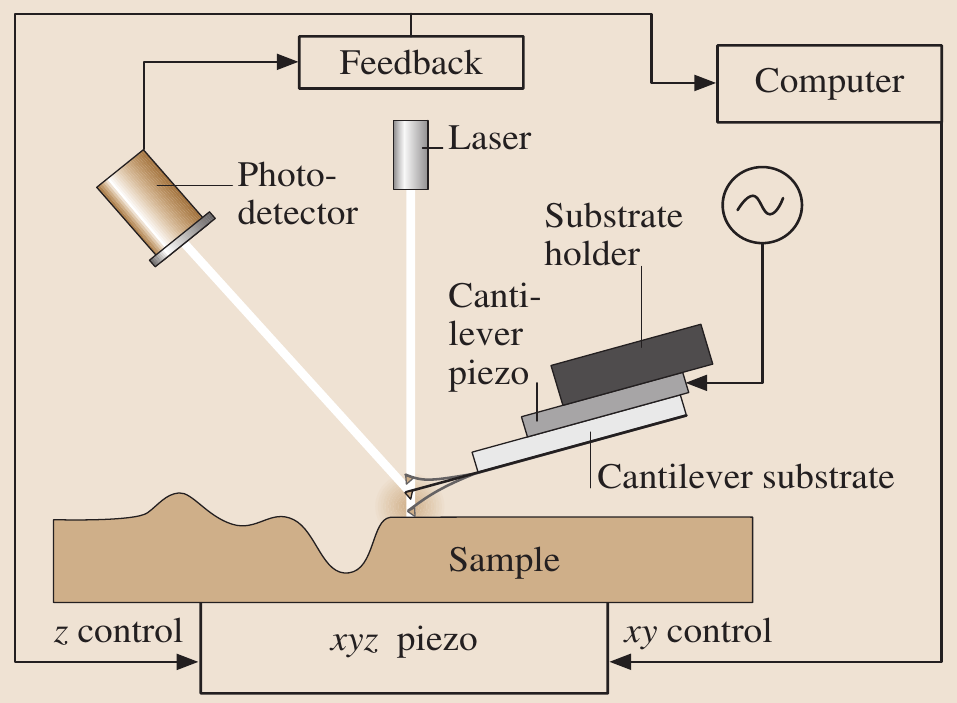
\includegraphics[width=0.5\textwidth]{Tapping_mode}
\caption{Schematic of tapping mode using a feedback mechanism to keep resonant frequency $\omega_0$ of the cantilever constant \cite{Bhushan}.}
\label{fig:Deflection_measurement}
\end{figure}

Similarly to the static mode, we can directly measure the force gradient or use this as a signal for a feedback mechanism that acts on the distance $r$ to keep constant the resonant frequency. An schematic draw is shown in Figure 

\subsection{NaioAFM}

\subsection{Gwyddion}


\section{Results and discussion}

\subsection{Static mode}

\subsubsection{Callibration}

\subsection{Tapping mode}

\subsubsection{Callibration}


\section{Conclusions}


\nocite{*}
\newpage
\bibliographystyle{unsrt}
\bibliography{references}


\end{document}